\lettrine[findent=0.4em, nindent=0em]{\textbf{P}}{robabilistic analysis} of
electronic systems is an extensive and diverse area, which is expanding with an
accelerating pace. The rapid growth is instigated by the fact that electronic
systems naturally become more sophisticated and refined, and that they penetrate
deeper into everyday life. Consequently, the impact of uncertainty inevitably
becomes more prominent and engender more severe consequences, necessitating an
adequate treatment. Therefore, the designer of electronic systems has to account
for the presence of uncertainty in order to develop efficient and reliable
products.

In order to account for uncertainty, one has to quantify it first. Uncertainty
quantification is a wide umbrella, and the corresponding techniques can deliver
radically different pieces of information about the quantity of interest. In
this paper, we are interested in probability distributions rather than, for
instance, corner cases. Designing for the worst case is often a poor solution as
the system at hand might easily end up being too conservative, overdesigned
\cite{quinton2012}. The value of probability distributions is well understood,
and it is especially high in the context of soft real-time systems and control
systems.

When it comes to uncertainty quantification and estimation of probability
distributions, Monte Carlo (\abbr{MC}) methods are of great use. Compared to
other techniques for probabilistic analysis, such methods are straightforward to
apply. The system at hand is treated as being completely opaque, and it only
needs to be simulated a number of times, following an adequate strategy, in
order to start drawing conclusions about the system's behavior. Consider, for
instance, the classical \abbr{MC} sampling, which is arguably the most famous
and versatile approach to the analysis of stochastic systems. The technique was
introduced in the middle of the twentieth century and since then has expanded
into a rich family of methods that have had a tremendous impact both in academia
and in terms of industrial breakthroughs.

The major problem with sampling techniques, however, is in sampling: one should
be able to obtain sufficient many realizations of the quantity of interest in
order to be able to draw sound conclusions with respect to that quantity
\cite{diaz-emparanza2002}. The main concerns here are: How many samples do we
need? How many samples can we afford? How long does it take to obtain one
sample? How much does one sample cost? When the subject of the analysis is
expensive---as measured by the metric that makes the most sense to the problem
at hand---computer experiments are rendered as slow and often infeasible.

We propose a system-level framework for the analysis of electronic systems that
are dependent on uncertain parameters. Similar to \abbr{MC} methods, our
technique treats the system at hand as a ``black box'' and, hence, is
straightforward to apply since no handcrafting is required and existing codes
need no change. Consequently, the quantities that the framework is able to
analyze are diverse; examples include the end-to-end delay, energy consumption,
and thermal dynamics of an application running on a multiprocessor system. In
contract to \abbr{MC} methods, our technique explores the structure of the
problem---that is, the dependence of the quantity of interest on the uncertain
parameters---by exercising the ``black box'' at a set of points chosen
adaptively. The adaptivity allows for reduction of the costs associated with the
system's evaluation. The magnitude of reduction depends on the problem, and it
can be substantial when the problem is well disposed to adaptation. Furthermore,
the adaptivity that our framework leverages is purely local, as opposed to the
dimension-wise adaptivity \cite{klimke2006}, which means that the framework can
benefit even further from the particularities of the stochastic space that are
not necessarily aligned with the stochastic dimensions. Lastly, the output of
our framework is generative: we construct a light representation of the quantity
of interest that can be used to generate realizations of this quantity without
touching the expensive ``black box.'' Therefore, having constructed such a light
representation, the \abbr{MC} machinery applies and has a practically negligible
cost.

In addition to the cost reduction mentioned earlier, the adaptivity featured by
the proposed framework means that our technique is well suited for nonsmooth
response surfaces. The ability to tackle nonsmooth problems is important for the
designer of electronic systems, and we would like to unpack this aspect now. To
this end, we first need to give a classification of sources of uncertainty
present in electronic systems.

Sources of uncertainty can be divided into analog and digital. The major
representative of the former is process variation \cite{srivastava2005}, which
has been central for many lines of research \cite{bhardwaj2008, juan2012,
lee2013, ukhov2014, ukhov2015}. Process variation is a side effect of the
fabrication process. In contrast, the sources of uncertainty labeled as
``digital'' are phenomena of the digital world rather than physical. To
elaborate, many applications running on modern devices exhibit nondeterministic
behavior: their characteristics change from one activation to another, depending
on such aspects as the runtime environment and input data. The digital class has
not been deprived of attention either, especially in the real-time community
\cite{quinton2012, diaz2002, santinelli2011, yang2013, tanasa2015}. Both analog
and digital sources of uncertainty render the behavior of electronic systems as
essentially random for the designer, and accounting for them can be highly
beneficial if not essential.

\begin{figure}
  \centering
  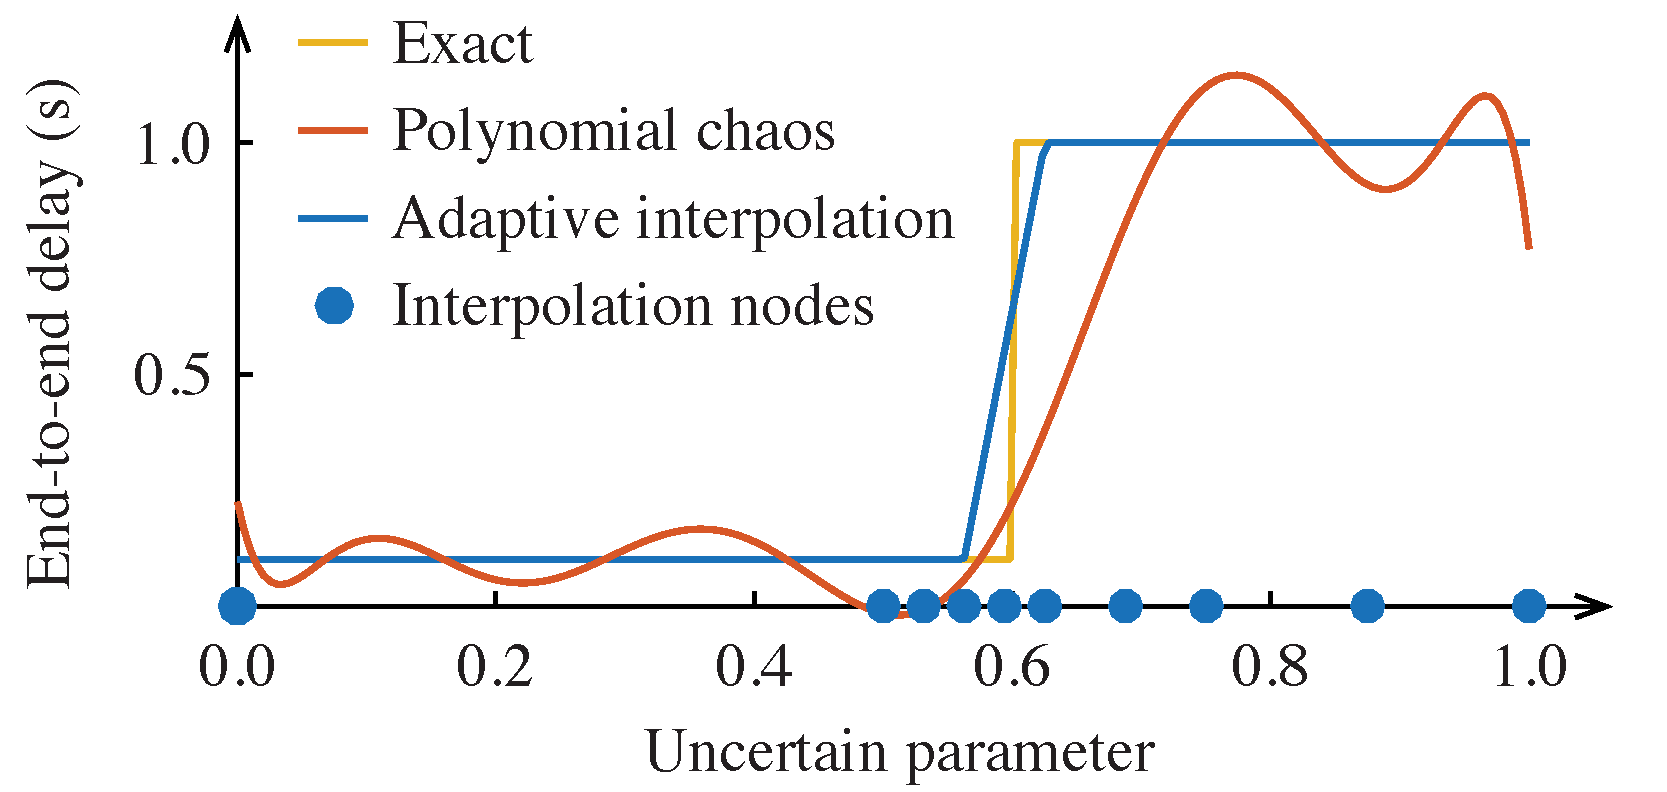
\includegraphics[width=1.0\columnwidth]{include/assets/figures/motivation.pdf}
  \caption{
    A motivational example.
  }
  \flab{motivation}
\end{figure}

Due to the physical nature, the variability induced by analog sources of
uncertainty is typically smooth. In such cases, uncertainty quantification based
polynomial chaos (\abbr{PC}) expansions \cite{xiu2010} and other global
approximations relying on polynomials generally works well, as in
\cite{bhardwaj2008, lee2013, ukhov2014, ukhov2015}. On the other hand, the
variability induced by digital sources of uncertainty often lacks smoothness and
might even have discontinuities. In such cases, \abbr{PC} expansions and similar
techniques fail. In order to explore this concern, let us consider a toy
example. Suppose that our electronic system has only one processing element, and
it is running an application with only one task. Suppose further that the task
has two branches and takes either of them depending on the input data. Assume
that one branch takes 0.1~s to execute and has probability 0.6, and the other
branch takes 1~s and has probability 0.4. Our goal is to find the distribution
of the end-to-end delay of the application. In this example, the end-to-end
delay coincides with the execution time of the task; hence, we already know the
answer. Let us pretend we do not and try to find it.

Suppose the above scenario is modeled by a random variable $\u$ uniformly
distributed in $[0, 1]$: the execution time of the task is 0.1~s if $\u \in [0,
0.6]$, and it is 1~s if $\u \in (0.6, 1]$. The response in this case is a step
function, which is illustrated by the yellow line in \fref{motivation}. First,
we try to quantify the end-to-end delay by constructing a \abbr{PC} expansion
founded on the Legendre polynomial basis \cite{xiu2010}. The orange line in
\fref{motivation} shows a ninth-order \abbr{PC} expansion, which uses 10 points.
It can be seen that the approximation is poor, not to mention negative
end-to-end delays. The observed oscillating behavior is the well-known Gibbs
phenomenon, stemming from the steepness of the response. Now we let our
framework make use of the same number of points as the \abbr{PC} expansion did.
The result is the blue curve in \fref{motivation}, and the adaptively chosen
points are plotted on the horizontal axis. It can be seen that the approximation
is good, and, in fact, it would be indistinguishable from the true response with
a few additional points. One can also note that the adaptive procedure started
to concentrate points at the jump and left the insipid regions on both sides of
the jump with no particular attention. Having constructed such an accurate
representation, one can proceed to the calculation of the probability
distribution of the quantity of interest, which, in general, is done via
sampling followed by such techniques as kernel density estimation. The crucial
point to note here is that this follow-up sampling does not involve the analyzed
electronic system itself and, thus, costs nothing.

The remainder of the paper is organized as follows. Section~\ref{sec:prior-work}
provides an overview of the prior work. In \sref{present-work}, we summarize the
contribution of the present paper. Preliminaries are given in
\sref{preliminaries}. The problem that we address is formulated in
\sref{problem-formulation}, and our solution to the problem is outlined in
\sref{solution}. The proposed framework is presented in \sref{modeling},
\sref{interpolation}, and \sref{analysis}. The experimental results are reported
and discussed in \sref{experimental-results}. Section \ref{sec:conclusion}
concludes the paper.
